\section{Biomedical sensing}
\subsection{\label{sec:level1}Magnetoencephalography}
\begin{figure}[b]
\centering
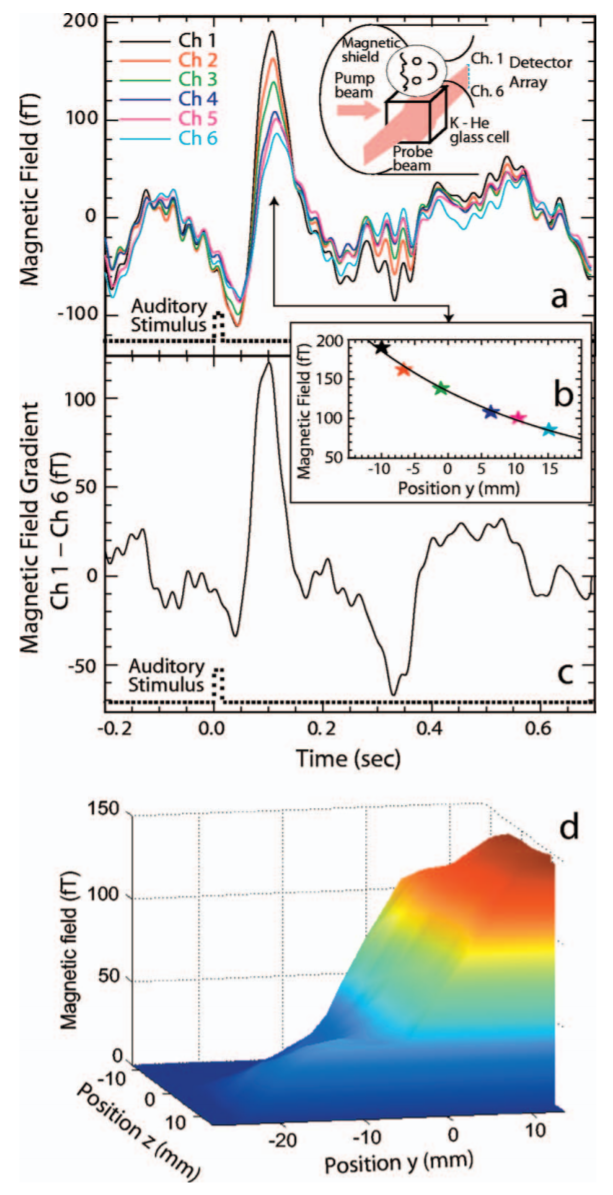
\includegraphics[height=0.7\textwidth,keepaspectratio]{MEG1}
\caption{\label{fig:MEG1} (a) Magnetic field detection averaged over 600 auditory stimuli. (b) The magnetic field gradient resulting from the difference in the position of the 6 channel photodiode which are each separated by 5mm. (c) Magnetic field gradient detection from the difference in the magnetic field signal between outer photodiode detectors in the vertical array. (d) Magnetic field detection using a 2D photodiode array \citep{XiaMagnetoencephalographyMagnetometer}.}
\end{figure}

This section discusses the schemes used and experimental results of employing a SERF AM in place of a SQUID magnetometer to complete mapping and detection of the magnetic fields produced by the human brain. In Ref. [\citen{XiaMagnetoencephalographyMagnetometer}], the first experimental MEG AM scheme was implemented. The subject lay on a bed and had their head secured above a 422 cm$^{3}$ potassium (K) vapor cell heated to 180$^{\circ}$. Between the subject and the heated vapor cell is a layer of insulating material and a water-cooling pad. The distance between the probe beam and the cooled surface is 2.5 cm. The bed is surrounded by three layers of magnetic shielding, generated by computationally controlling the magnetic fields induced by 18 coils, with an opening to fit the subjects head. 


The biomagnetic field is measured by detecting the rotation of the linearly polarised light. Prior to being detected by a 6 channel photodiode array, the linearly polarised probe light passes through polarising beam splitter orientated such that light intensity detected increases as the polarisation plane is rotated. The magnetometer is initially calibrated by applying a magnetic field which is used to measure the 3.5 fTHz$^{-1/2}$ sensitivity of the magnetometer at 10 Hz. The laser intensity fluctuations are attributed to the 1/$f$ noise spectrum. The averaged results of applying a single train of 16, 1 ms period square-wave pulses to provide an auditory stimulus is shown in Fig. (\ref{fig:MEG1}a). Therefore, the brain response to the stimuli is observed by the large peak in the magnetic field detection. The dependence on the spatial position of the photodiode detector is highlighted in Fig. (\ref{fig:MEG1}b,c). The possibility of mapping the region of the brain activated by the stimuli is illustrated in Fig. (\ref{fig:MEG1}d) where a 2D photodiode detector array is used.

\begin{figure}[b]
\centering
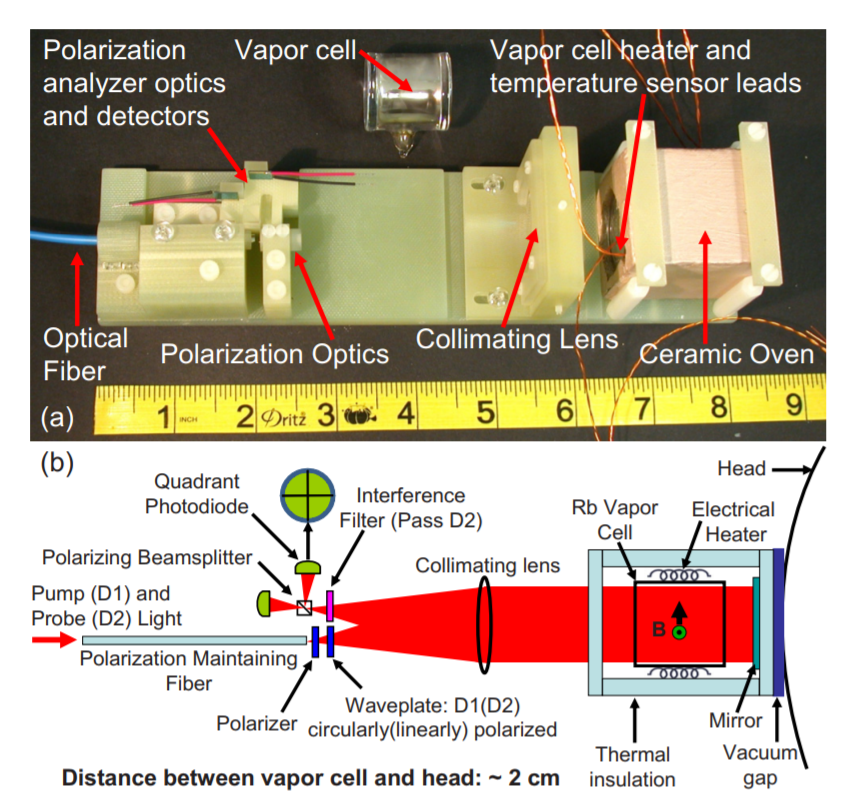
\includegraphics[height=0.4\textwidth,keepaspectratio]{MEG2a}
\caption{\label{fig:MEG2a} Atomic magnetometer (a) device photograph and (b) optical set-up. The laser field operates on a single optical axis which produces a circularly polarised D1 pump beam and linearly polarised D2 probe beam. The horizontal and vertical polarisation components of the probe are detected by separate quadrant photodiodes after the beam has been reflected back through the vapor cell \citep{Johnson2010MagnetoencephalographyMagnetometer}.}
\end{figure}

The fiber-coupled rubidium (Rb) AM shown in Fig. (\ref{fig:MEG2a}) was developed and used to complete a study of the response a subjects brain to, auditory and median nerve, stimuli which are compared to the results when using a commercial SQUID system in Ref. [\citen{Johnson2010MagnetoencephalographyMagnetometer}]. The device and has a measured sensitivity of $<$5 fTHz$^{-1/2}$ between 5-10 Hz and the subject is 2cm from the center of the cell. To increase the atomic number density to the SERF regime the cell is heated to 190 $^{\circ}$ and thermally isolated from the subject. The circularly polarised pumping enables sensitive detection of the perpendicular $B$ field where lock-in detection of the probe beam polarisation is produced using a perpendicular 1kHz modulated magnetic field. The study was completed in a shielded room where the AM required further $B$ field canceling which is achieved similarly as previously discussed for the AM design in Ref. [\citen{XiaMagnetoencephalographyMagnetometer}]. The magnetic field signal generated from the left side of the brain is detected as shown in Fig. (\ref{fig:MEG2b}).  

\begin{figure}[b]
\centering
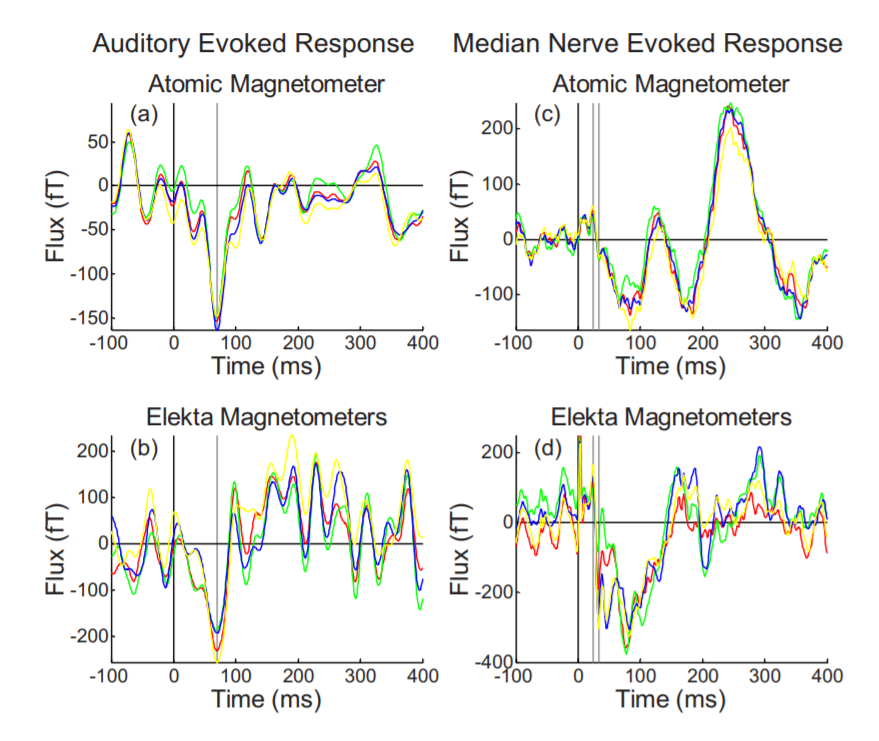
\includegraphics[height=0.43\textwidth,keepaspectratio]{MEG2b}
\caption{\label{fig:MEG2b} Magnetic flux (a) auditory and (c) right median nerve response measured by a quadrant 4-channel AM. Magnetic flux (a) auditory and (c) right median nerve response measured by four SQUIDs located near the position of the AM. The stimuli are applied at time $t=0$ s and the vertical grey lines illustrate times at which these commonly used stimuli are expected to induce responses \citep{Johnson2010MagnetoencephalographyMagnetometer}.}
\end{figure}

\begin{figure}[t]
\centering
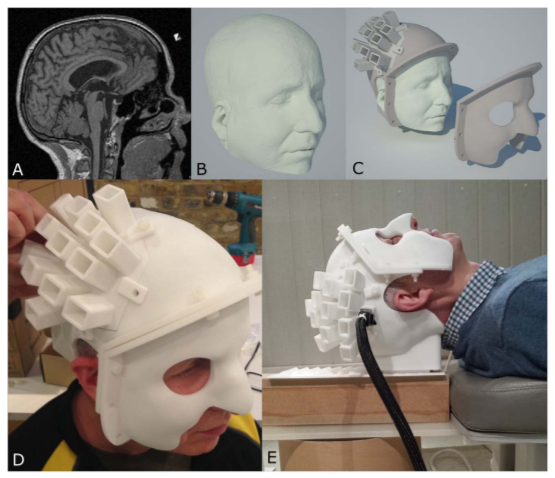
\includegraphics[height=0.4\textwidth,keepaspectratio]{MEG4a}
\caption{\label{fig:MEG4a} 3D head-cast fabrication. (a) MRI slice and (b) MRI reconstruction provided precise measure of subjects head. (c) Computer-aided design of head-cast with AM connectors for measurements of brain activity in the sensorimotor cortex. (D) The subject is wearing the 3D printed head-cast and (E) the AM attached is attached during experiment \citep{Boto2017AMagnetometers}.}
\end{figure}


The right median nerve is stimulated by a 0.8 mA electrical pulse of duration 200 $\mu$s applied to the subjects right arm and 1 kHz pulse of duration 0.25 s was used to stimulate the left audio cortex. The time between pulses is varied and the bandpass filters are used to reduce frequency noise. The magnetic field component that SQUIDs measure is perpendicular to the subject's head which is different from the component that the AM detects. Additionally the AM 4 channel detection separation is 5 mm which is smaller since the 4 SQUIDs are separated by 30 mm. Therefore, the responses which occur around 100 ms have an acceptable level of agreement and verifies that the AM has potential to provide a non-cryogenic and cheaper alternative for producing MEG systems.  

The chip-scale AM in Ref. [\citen{Sander2012MagnetoencephalographyMagnetometer.}] has a one beam optical axis but has separate optical fibers used to transmit the light to the 2 mm$^{2}$ vapor cell and from the vapor cell to the detector. The reduction in size of the device produces a reduction of the sensitivity to 200 fTH$^{-1/2}$ between 5-150 Hz. The AM measured the biomagnetic field response of the occipital region and left somatosensory cortex when the subject opens and closes their eyes and when the right median nerve is stimulated, respectively. Again the results are verified by comparison with a commercial SQUID array. AM sensitivity of $\approx$ 3 fTH$^{-1/2}$ should be attainable for this device and an increase from the 30 $\%$ efficiency of light detection will significantly improve the sensitivity. 

In Ref. [\citen{Shah2013AApplications}] an AM is presented with a similar design as in Ref. [\citen{Sander2012MagnetoencephalographyMagnetometer.}] but with a larger vapor cell and enclosed by a 50 cm$^{3}$ 3D printed casing made from plastic which can withstand the 190 $^{\circ}$ cell temperature. Magnetic coils wrapped round the thermally isolated layer remove residual magnetic fields in a magnetically shielded room. AM MEG and MCG was completed for auditory and somatosensory stimuli, respectively. The sensitivity of the AM was 10 fTHz$^{-1/2}$ when completing MEG. The significant improvement in the sensitivity of the device is attributed to the increased S/N due to the average distance between the subject and the AM surface being $<$1 cm at a frequency bandwidth of 100 Hz. 
\begin{figure}[b]
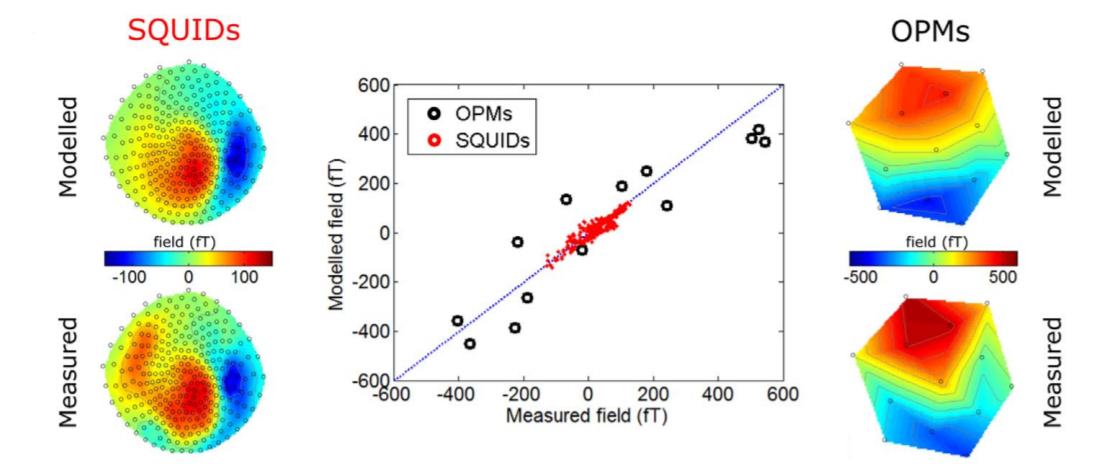
\includegraphics[height=0.23\textwidth,keepaspectratio,]{MEG5}
\caption{\label{fig:MEG5} SQUID and AM modeled and measured 2D tomographic response to the somatosensory stimuli. The center plot shows the comparison between the modeled field and the measured data \citep{Boto2017AMagnetometers}.}
\end{figure}
A similar AM device design as in Ref. [\citen{Shah2013AApplications}] was used in a study in Ref. [\citen{Boto2017AMagnetometers}] where 3D printing produced a subject specific MEG head-cast. The fabrication process is illustrated in Fig. (\ref{fig:MEG4a}). The optimum position of the 13 AMs for detection of sensory and motor response to stimuli is determined from data collected using a 275-channel commercial SQUID system. The left median nerve is stimulated using electrical pulses with a current amplitude set such that the subject's thumb twitches when the pulse is applied. Mapping of the magnetic field in response to the automotive stimuli is shown in Fig. (\ref{fig:MEG5}) for the AM and SQUID sensors. The 13-channel AM array is obtained by repeating experiment 13 times with the AM in a different position each time. The modeled tomography removes environmental interference by generating a computation gradiometer array from the measured AM and SQUID data. The computational gradiometer successfully removes the mains peak frequency in the AM detection array and the corrected sensitivity is 15.9 fTHz$^{-1/2}$ with a bandwidth > 100 Hz. The agreement between the AM modeled and measured $B$ field is very promising considering the use of only one AM to produce a 13 channel array. The AM has a dynamic range of ± 5 nT for operation in the SERF regime.
\subsection{Magnetic Induction Tomography}
Atrial fibrillation is a heart condition which is characterised by an irregular heart rate which produces abnormal conductivity of the heart tissue. Development of an noninvasive technique to diagnose and treat this condition, and possibly detect malignant tissue, using conventionality MIT has previously been unsuccessful \citep{Marmugi2016OpticalHeart}. In the conventional MIT scheme a magnetic field is generated from current flowing through the primary coil. The magnetic field induces an Eddy current in the sample material and a secondary coil is used sense the conductivity. However, the conductivity of the biological material is very small which limits the ability detect the magnetic field induced \citep{Griffiths2001MagneticTomography}. 






A noval MIT scheme has been developed in Ref.[\citen{Deans2016ElectromagneticMagnetometer}] which uses an all optical pump-probe AM and applies an rf magnetic field to drive atoms from the Dark states. The result is rf polarisation rotation of the probe beam. Therefore changes in the phase or amplitude of the detected probe light due to Eddy currents in the biological tissue enables mapping of tissue conductivity. In Ref. [\citen{Deans2016OpticalHeart}] the dynamic range of the sensing device is illustrated by completing MIT of metal samples where the known conductivity of one sample is two orders of magnitude larger than the other. The future implication for diagnosing heart conditions, of accurate MIT regardless of the sample conductivity, is highlighted in Fig. (\ref{fig:MIT}).

\begin{figure}[h]
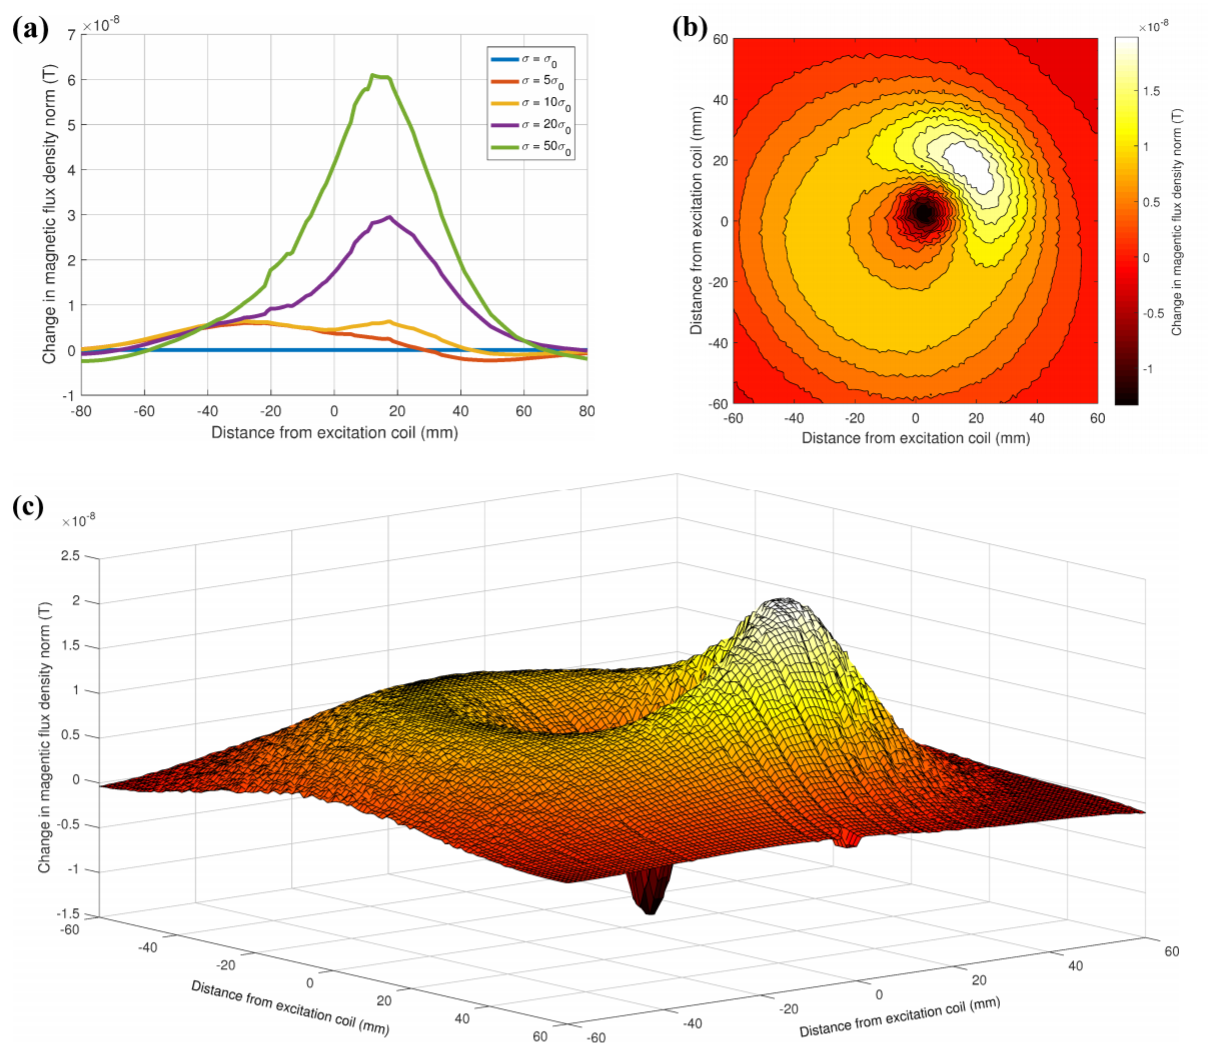
\includegraphics[height=0.42\textwidth,keepaspectratio,]{MIT}
\caption{\label{fig:MIT}(a) Change in the magnetic flux due to due variation in anomaly conductivity, where $\sigma_{0}=0.875 Sm^{1}$. Heart anomaly contour plot in (b) 2D and (c) 3D \citep{Deans2016OpticalHeart}.}
\end{figure}

